\chapter{Realizace}

\begin{chapterabstract}
Tato kapitola popisuje jednotlivé fáze vývoje aplikace, která slouží k~tvorbě interaktivních vzdělávacích materiálů. 
Nejprve je představen iterativní přístup, který umožnil průběžné testování a úpravy na základě zpětné vazby. 
Dále jsou rozebrány technické aspekty realizace -- od struktury klientské a serverové části, přes návrh a implementaci editoru a přehrávače, až po možnosti lokalizace, responzivity a zabezpečení. 
Kapitola se rovněž věnuje systémům rozšíření, multimédiím a uživatelským interakcím, které tvoří základ pro škálovatelnost a budoucí rozvoj platformy. 
Nakonec kapitola ukazuje nasazení platformy společně s~tím, co se pro platformu vytvořilo a co je možné s~pomocí aplikace vytvořit za materiály.
\end{chapterabstract}

\section{Tvorba prototypu}


Během výběru samotného zadání této diplomové práce bylo nutné zvážit řadu faktorů, které by mohly ovlivnit realizovatelnost navrhovaného řešení. 
Jedním z~klíčových aspektů byl potenciální problém s~editorem, který by měl sloužit jako základ pro interaktivní tvorbu vzdělávacích materiálů. 
Jelikož existovalo riziko, že požadovanou funkcionalitu nebude možné efektivně implementovat v~dostupných technologiích, bylo rozhodnuto o~vytvoření prototypu. 
Tento prototyp měl za cíl ověřit proveditelnost hlavních funkcí a eliminovat případné zásadní překážky v~rané fázi vývoje.

V rámci tvorby prototypu byly implementovány a testovány různé způsoby vykreslování obsahu, přičemž klíčovou otázkou bylo, zda bude vhodnější využít technologii HTML, SVG nebo Canvas.
Každý z~těchto přístupů má své specifické výhody a nevýhody, které ovlivňují, jak kvalitu zobrazení, tak výkon a možnosti interakce s~uživatelem. 
Podrobnější rozbor těchto technologií je uveden v~sekci~\ref{text:vykreslovani}, kde jsou jednotlivé přístupy porovnány z~hlediska efektivity a použitelnosti v~kontextu plánované platformy.

Při vývoji prototypu se objevily i~obecné problémy související s~implementací editoru -- respektive s~jejich matematickou reprezentací. 
Klíčovou výzvou se ukázaly být skupinové transformace a manipulace s~prvky na plátně, zejména pokud jde o~jejich pohyb a transformaci v~rámci editačního prostoru.
Bylo nutné vyřešit, jakým způsobem budou tyto operace realizovány tak, aby editor zůstal uživatelsky přívětivý, efektivní a zároveň umožňoval pokročilé úpravy vytvořeného obsahu.

Na základě získaných poznatků byl prototyp úspěšně dokončen a posloužil jako důkaz, že zamýšlená funkcionalita může být realizována v~rozumném stavu. 
Tento krok umožnil přejít k~další fázi vývoje, která se zaměřuje na návrh a implementaci finální verze platformy s~důrazem na rozšiřitelnost, komunitní podporu a snadnou použitelnost pro pedagogy i~studenty.

Prototyp sloužil především k~ověření základního konceptu a nebyl určen pro přímé použití v~konečné implementaci platformy. 
Jeho účelem bylo rychlé experimentování s~klíčovými funkcionalitami, bez důrazu na optimalizaci kódu či dlouhodobou udržitelnost. 
Po potvrzení, že zamýšlené principy mohou fungovat, bylo nutné přistoupit k~přepsání prototypu do robustní a udržitelné podoby. 
Tento krok zahrnoval refaktorování kódu, zpřehlednění architektury a návrh struktury, která umožní snadnou údržbu i~budoucí rozšíření funkcionalit. 
Přepis zároveň eliminoval technické dluhy vzniklé při rychlém vývoji.

\section{Metodika vývoje}\label{text:realizace/metodikaVyvoje}

Proces vývoje platformy pro tvorbu interaktivních výukových materiálů probíhal iterativním způsobem, což umožnilo průběžné testování a úpravy jednotlivých částí aplikace. 
Tento přístup se ukázal jako efektivní nejen při samotné implementaci, ale i~při optimalizaci uživatelského prostředí na základě zpětné vazby od testerů.

Vývoj začal základním návrhem a analýzou požadavků, což bylo detailně popsáno v~kapitolách~\ref{text:navrh} a~\ref{text:analyza}. 
Po definování architektury systému a stanovení klíčových funkcionalit byl zahájen samotný vývoj. 
Každá část aplikace byla pečlivě promyšlena před jejím naprogramováním, přičemž se důraz kladl na modularitu a možnost budoucího rozšíření.

Samotný vývoj probíhal iterativně. 
V každém cyklu bylo nejprve rozhodnuto, na které části aplikace se bude pracovat. 
Poté následovala detailní analýza a návrh této části, což umožnilo identifikovat možné komplikace ještě před samotnou implementací. 
Po naprogramování byla nová funkcionalita nasazena na dočasné testovací prostředí, kde probíhalo její testování různými uživateli. 
K testování byli zapojeni především kolegové a studenti (viz kapitola~\ref{text:testovani}), jejichž zpětná vazba byla klíčová pro identifikaci problémů a návrh zlepšení.

Získané podněty byly zaznamenány a klasifikovány dle priority. 
Kritické chyby byly opraveny okamžitě, zatímco drobné úpravy a návrhy na zlepšení byly zařazeny do plánu budoucího vývoje. 
Tento přístup zajišťoval nejen stabilní vývoj systému, ale také jeho postupné vylepšování bez nutnosti výrazných zásahů do již implementovaných částí.

Během vývoje byl také kladen důraz na refaktoring kódu, což umožnilo udržovat čitelnost a efektivitu implementace. 
Starší části aplikace byly pravidelně přepisovány a optimalizovány s~cílem zvýšit výkon a usnadnit další rozšíření systému.

Tento iterativní proces vývoje umožnil nejen průběžné zdokonalování aplikace, ale také pružně reagovat na nové požadavky a potřeby uživatelů. 
Díky tomuto přístupu bylo možné zajistit vysokou kvalitu finální verze platformy a její snadnou škálovatelnost pro budoucí rozšíření.

Vývoj platformy probíhal v~prostředí verzovací služby GitLab, která sloužila jako hlavní nástroj pro správu kódu. 
Zároveň jsem využíval GitHub pro synchronizaci a zálohu repozitáře. 
Projekt byl veden jako monorepozitář, což umožnilo jednoduchou provázanost všech součástí systému, které spolu úzce souvisí. 
Tento přístup se ukázal jako výhodný pro počáteční vývoj, nicméně do budoucna by bylo vhodné jednotlivé části oddělit do samostatných repozitářů s~jasně definovaným rozhraním.

Pro lepší orientaci v~historii změn jsem používal sémantické zprávy. 
Každá zpráva jasně popisuje, co se změnilo a v~jaké části systému, což usnadňuje zpětné dohledávání konkrétních úprav. 
V rámci vývoje vzniklo přes 700 samostatných balíčků změn (tzv. commit), které pokrývají vývoj nových funkcí, opravy chyb i~refaktoring.

Plánování probíhalo mimo samotné verzovací nástroje, především prostřednictvím služby ClickUp. 
Tento nástroj sloužil ke správě úkolů, revizí a sledování pokroku ve vývoji. 
Pomáhal mi tak udržet přehled o~jednotlivých krocích, přestože jsem pracoval většinou samostatně.


\section{Klientská část}\label{text:realizace/klient}

Klientská část aplikace byla vyvinuta jako webová aplikace v~souladu s~návrhem ze sekce~\ref{text:navrh/klient}. 
Pro implementaci byl zvolen framework Vue spolu s~nástrojem Vite, který umožňuje rychlý vývoj a stabilní správu závislostí.

Pro usnadnění tvorby požadovaných funkcionalit bylo využito několika knihoven, které zajišťují specifické potřeby aplikace. 
Mezi klíčové patří:

\begin{description}
    \item[floating-vue] Slouží k~tvorbě vyskakovacích nápověd a kontextových menu.
    \item[moment] Umožňuje snadnou správu a manipulaci s~daty a časovými údaji.
    \item[pinia] Poskytuje jednoduchý a efektivní způsob správy globálního stavu aplikace.
    \item[vue-router] Umožňuje vytvoření více virtuálních stránek v~rámci jedné aplikace.
\end{description}

Dále byly použity i~další knihovny, které přispívají k~lepší modularitě a efektivitě vývoje.
O některých se budu dále zmiňovat v~následujících sekcích.

\subsection{Komponenty}

V souladu s~analýzou v~sekci~\ref{text:navrh/design/komponenty} byly vytvořeny všechny potřebné komponenty. 
Při jejich návrhu byl kladen důraz na znovupoužitelnost a udržitelnost kódu, přičemž značná část tvorby, inspirace a kódu pocházela z~mé bakalářské práce~\cite{cajthaml_bp}.

První iterace vývoje se zaměřovala na základní implementaci klíčových prvků a ověření jejich funkčnosti. 
Hlavním cílem bylo zajistit, aby komponenty byly dobře udržitelné a univerzálně použitelné v~různých částech aplikace.

Tyto komponenty sloužily především pro webovou stránku a uvnitř editoru (viz sekce~\ref{text:realizace/editor}) se nepoužívají.

\subsection{Designový návrh}

První verze designu aplikace využívala komponenty a vizuální prvky, které byly navrženy s~důrazem na rychlost vývoje a demonstraci funkčnosti. 
Tento přístup umožnil efektivní iteraci a testování uživatelského rozhraní v~raných fázích vývoje.
Komponenty vycházely z~designu vytvořeného v~rámci mé bakalářské práce, což přineslo nejen vizuální kontinuitu, ale i~možnost znovupoužití ověřeného kódu.

Postupem času bylo nutné design sjednotit a vytvořit konzistentní vizuální styl aplikace.
Namísto pevně daného návrhu jsem pracoval iterativně -- upravoval jsem komponenty, barvy a jejich proměnné, dokud celek nepůsobil harmonicky a esteticky vyváženě. 
Jako hlavní vizuální inspiraci jsem zvolil styl \texttt{glassmorphism}, který se vyznačuje průhlednými a rozmazanými prvky, čímž vytváří moderní a elegantní uživatelské rozhraní.
Tento styl je populární v~moderním UI/UX designu a využívají ho například operační systémy macOS a Windows~11 nebo některé mobilní aplikace.
Součástí vizuální identity aplikace se stala fialová barva doplněná o~gradienty, což přispívá k~výraznému a zapamatovatelnému vzhledu.

Hlavním cílem bylo vytvořit jednoduchý, ale vizuálně přitažlivý design, který bude snadno přizpůsobitelný.
Na obrázku~\ref{fig:realizace/design} je možné vidět ukázku implementovaných komponent a jejich designu.
Pro usnadnění budoucích úprav a možnou implementaci více barevných režimů byly ve stylování využity CSS proměnné.
Tento přístup umožňuje nejen jednoduché změny barevných schémat, ale i~potenciální rozšíření designu o~tmavý nebo kontrastní režim podle preferencí uživatele.



\begin{figure}[ht!]
    \centering
    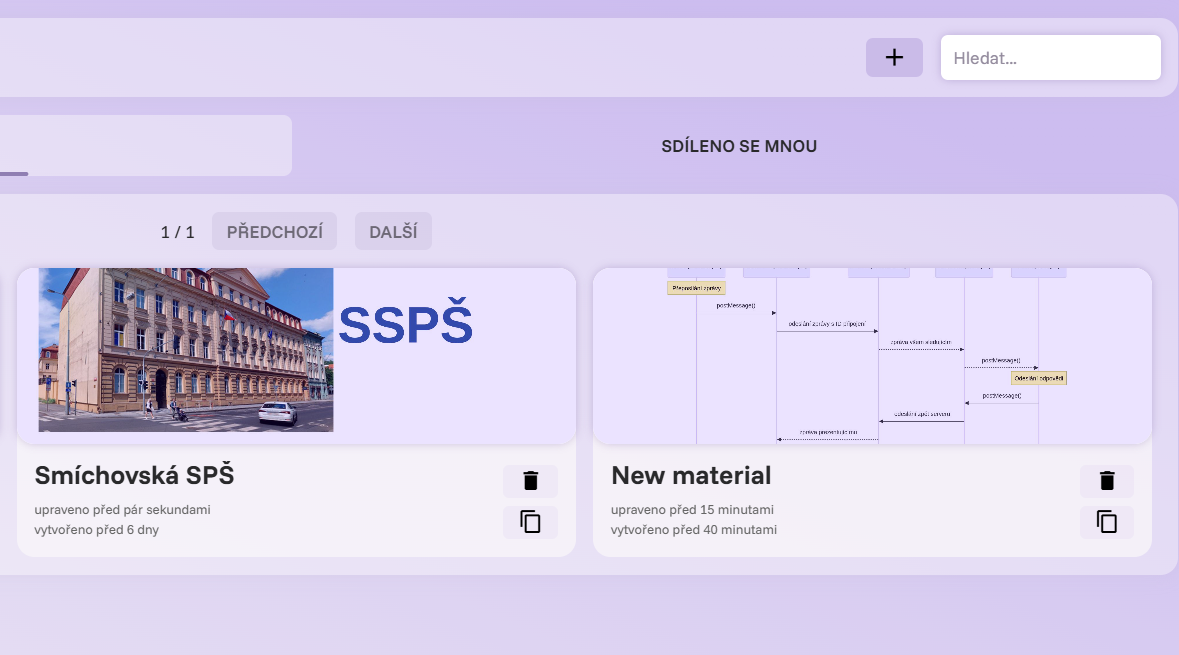
\includegraphics[width=0.8\textwidth]{media/05_realizace/design.png}
    \caption[Prvky v~implementovaném designu aplikace]{Prvky v~implementovaném designu aplikace, lze vidět kartu, tlačítko, vstupní pole, navigaci a stránkovač}
    \label{fig:realizace/design}
\end{figure}


\subsection{Autentizace a autorizace}

Aplikace odděluje obsah určený pro veřejnost od částí přístupných pouze přihlášeným uživatelům. 
Všechny stránky s~výjimkou přehrávače jsou dostupné jen po přihlášení. 
Autentizace probíhá pomocí tokenu, který se ukládá do \texttt{localStorage}. 
Pokud token vyprší, uživatel je automaticky přesměrován na přihlašovací obrazovku.

Autorizace se opírá o~kontrolu přístupových práv při každém požadavku. 
Při každém požadavku v~hlavičce \texttt{Authorization} s~typem \texttt{Bearer} nalezne řetězec kódu JWT.
Kód obsahuje mimo jiné ID a jméno uživatele pro rychlejší přístup v~aplikaci.

Pokud uživatel nemá oprávnění k~požadované akci nebo zdroji, server vrací chybu. 
Klient správně reaguje na neúspěšné požadavky vyskakovacími okny, dialogy a jinými upozorněními.

Každý materiál má svého vlastníka, který k~němu má vždy plný přístup. 
Vlastník materiálu může určit seznam spoluúčastníků, kteří mají přístup k~editoru a přehrávání materiálu.

Materiály dále rozlišují viditelnost pomocí příznaku \texttt{visibility}. 
Pokud je nastavena hodnota \texttt{PUBLIC}, je materiál veřejně dostupný pro přehrávání přes přehrávač. 
V opačném případě, tedy při hodnotě \texttt{PRIVATE}, je přístup omezený pouze na vlastníka a případně přidané spolupracovníky.

\subsection{Responzivita}\label{text:realizace/responzivita}


Všechny stránky aplikace jsou přizpůsobené pro různá zařízení, jak je podrobněji uvedeno v~kapitole~\ref{text:testovani}. 
Responzivita je zajištěna hlavně díky použití komponentového systému a systému gridu, přičemž konkrétně se využívá dvanácti sloupcového rozvržení. 
Rozdělení do sloupců je řízeno pomocí CSS tříd a breakpointů, přičemž nejčastěji se používají pouze tři základní -- \texttt{sm}, \texttt{md} a všechny vyšší velikosti.

Většina rozvržení se přizpůsobuje právě přes tyto nastavené breakpointy. 
Dále se využívají pomocné třídy pro nastavení okrajů (\texttt{margin}), vnitřních okrajů (\texttt{padding}), flexibilního rozmístění prvků (\texttt{flex}) a rozestupů (\texttt{gap}). 
Tyto třídy také reagují na breakpointy, což umožňuje jemné doladění vzhledu jednotlivých částí rozhraní podle šířky obrazovky.

Výjimku tvoří editor, který má z~pohledu responzivity specifické chování. 
Podrobnosti jeho řešení jsou popsány v~sekci~\ref{text:realizace/editor}. 
V jeho případě bylo nutné upravit některé části individuálně, protože běžné techniky nebyly dostačující.

\subsection{Překlady}

Překlady v~aplikaci probíhají pomocí vlastního systému, který vychází ze strukturovaného zápisu v~jazyce JSON. 
Každý překlad je identifikován unikátním klíčem, například \texttt{editor.action.delete.tooltip}, a může být uložen ve stromové struktuře. 
V kódu~\ref{code:zapisPrekladu} jsou vyobrazeny zápisy překladů.
Tento přístup zajišťuje přehlednost a snadnou údržbu jednotlivých jazykových mutací.


\begin{listing}[ht!]
\caption{Zápisu překladů}\label{code:zapisPrekladu}
\begin{minted}{json}
{
  "editor": {
    "action": {
      "delete": {
        "tooltip": "Delete"
      },
      "add.tooltip": "Add"
    }
  }
}
\end{minted}
\end{listing}

K překladu textů v~rozhraní se využívají direktivy \texttt{v-t} a funkce \texttt{\$t}, které dovolují překlad.
Taktéž umožňují vkládání proměnných přímo do přeložených řetězců. 
Proměnné jsou nahrazovány pomocí syntaxe jako \texttt{\%test\%}, což umožňuje dynamickou práci s~obsahem bez nutnosti duplicitních překladů.

Aktuálně aplikace podporuje dva jazyky: češtinu a angličtinu. 
Překlady se ukládají i~do zkrácené podoby v~URL, což umožňuje přímé sdílení konkrétní jazykové verze rozhraní. 
Do budoucna lze očekávat problémy spojené se skloňováním, zejména v~jazycích se složitou gramatikou, která vyžaduje flexibilitu podle kontextu. 
Tento aspekt zatím systém neřeší a může být řešen později například pomocí rozšíření stávající logiky.

\subsection{Optimalizace pro webové vyhledávače}

Klientská část platformy je postavena jako SPA pomocí frameworku Vue. 
Tento přístup přináší některé výhody z~hlediska vývoje a uživatelského zážitku, ale současně komplikuje indexaci obsažených stránek vyhledávacími nástroji. 
Problém spočívá v~tom, že většina obsahu se vykresluje až po načtení skriptů, což někteří roboti vyhledávačů nezohlední.

Tento problém byl vyřešen pomocí techniky \textit{prerendering}.
Při detekci specifického \textit{user-agent} (typicky pro vyhledávací roboty) je požadavek přesměrován na službu \texttt{prerender}, která spustí virtuální prohlížeč, vykreslí cílovou stránku a vrátí její výsledný HTML výstup.
Výsledkem je obsah, který lze snadno indexovat bez ohledu na způsob zobrazení na straně klienta.

Z hlediska obsahu je pro SEO zásadní zejména přehrávač, který obsahuje samotné výukové materiály, a přihlašovací stránka. 
Prerendering je nasazen také pro hlavní stránku platformy, jak je popsáno v~sekci~\ref{text:realizace/hlavniStranka}. 
Samotné nasazení této služby je detailně popsáno v~sekci~\ref{text:realizace/nasazeni}.

Pro zlepšení optimalizace na straně klienta se používá knihovna \texttt{unhead}, která umožňuje dynamicky upravovat nadpisy stránek a další SEO metadata. 
V kombinaci s~prerendering tak vzniká systém, který je pro vyhledávače čitelný a současně neomezuje funkčnost platformy. 
Stránky jsou navíc přístupné a plně responzivní, jak rozvádím v~sekci~\ref{text:realizace/responzivita}.

Alternativa k~tomuto by byla použít vykreslování na serveru pomocí nějakého frameworku, třeba Nuxt.
Vzhledem k~tomu, že stránky nejsou takovým velkým cílem SEO, zdála se mi tato možnost jako nevhodná, a proto jsem ji nezvolil.

\section{Serverová část}\label{text:realizace/server}

Serverová část aplikace byla implementována v~souladu s~návrhem popsaným v~sekci~\ref{text:navrh/server}. 
Hlavním jazykem byl TypeScript a vývoj probíhal s~využitím frameworku Nest. 

Pro jednotlivé funkce byly použity následující balíčky:

\begin{description}
    \item[bcrypt] Kvalitní hashovací funkce, pro ochranu hesel.
    \item[class-validator] Pro validaci příchozích dat.
    \item[mjml] Pro formátování e-mailových šablon
    \item[puppeteer] Pro spouštění virtuálního prohlížeče pro generování náhledových obrázků a exporty materiálů.
    \item[nodemailer] Pro odesílání e-mailů.
    \item[socket.io] Pro správu WebSocketů, tedy real-time komunikace.
\end{description}

Nest framework je ve výchozím stavu postaven na knihovně Express a s~tím jsem počítal i~v~návrhu aplikace.
V tomto projektu byl ale nakonec nahrazen za Fastify, protože Nest podporuje přepnutí serverového procesoru nativně. 
Změna nevyžadovala větší úpravy a přinesla drobné výhody z~hlediska výkonu a např. nahrávání souborů.

V porovnání s~klientskou částí byla implementace serveru časově méně náročná.
Nejvíce úsilí vyžadovala klientská část, respektive vývoj editoru a přehrávače, jejichž návrh i~funkcionalita byly složitější.

\subsection{Moduly}

Nest klade důraz na modularitu. Každá část aplikace je definována jako samostatný modul. V~projektu byly vytvořeny tyto moduly:

\begin{description}
    \item[materials] -- správa výukových materiálů a jejich export.
    \item[auth] -- registrace, přihlašování a správa autentizace.
    \item[email] -- odesílání e-mailů a jejich šablonování.
    \item[data-export] -- zpracování a přijímání požadavků pro vygenerování balíčku osobních dat z~projektu.
    \item[events] -- real-time komunikace, kolaborace na materiálech a sledování materiálů.
    \item[plugin] -- správa rozšíření a jejich verzí.
    \item[media] -- správa mediálního obsahu uživatelů. 
    \item[preferences] -- správa uživatelského nastavení a personalizace.
    \item[users] -- uživatelské účty a jejich metadata.
\end{description}

Moduly \texttt{media}, \texttt{users}, \texttt{preferences} a další využívají knihovnu Mongoose pro práci s~databází MongoDB. 
Schémata jednotlivých entit byla vytvořena již v~době návrhu, v~implementaci byly zjištěny různé nedostatky z~původního návrhu a bylo nutné některé entity změnit.

\subsection{Autentizace a autorizace}

Autentizační logika využívá tzv. \emph{guards}, které Nest nabízí jako mechanismus pro kontrolu přístupu.
Guardy se aktivují pomocí TS dekorátorů a lze jimi snadno řídit, které části systému vyžadují přihlášení a jakým způsobem. 
Použity byly různé varianty guard -- pro běžné API volání, volitelnou autentizaci a také specifické guard pro připojení WebSocket.

Autorizace není centralizovaná, ale probíhá na úrovni jednotlivých koncových bodů. 
V každém případě se ověřuje, zda má uživatel přístup k~danému materiálu -- buď je veřejný, nebo je uživatel jeho vlastníkem, případně účastníkem kolaborace.

\subsection{Přenos a výměna dat}

Komunikace mezi serverem a klientem probíhá pomocí formátu JSON.
Pro strukturovaný přenos dat byly vytvořeny DTO třídy, které definují, jaká data se mají mezi klientem a serverem přenášet. 
Tyto DTO se využívají, jak v~serverové, tak klientské části aplikace, což vyžadovalo častou synchronizaci během vývoje.

Validace těchto objektů probíhá pomocí knihovny \texttt{class-validator}, která umožňuje definovat validační pravidla přímo v~kódu tříd.
V kódu~\ref{code:realizace/dto} je ukázka DTO s~validací.
To přispívá ke konzistenci a zajišťuje, že na server se nikdy nedostanou nevalidní data přímo z~klientské části.


\begin{listing}[ht!]
\caption[DTO s~validací pro přihlášení]{DTO s~validací pro přihlášení, \textit{kód zkrácen a modifikován pro přehlednost}}\label{code:realizace/dto}
\begin{minted}{typescript}
export default class InAuthDTO {
    @IsIn(['EMAIL_PASSWORD', 'EMAIL'])
    type: 'EMAIL_PASSWORD' | 'EMAIL';
    /**
     * The email address of the user.
     */
    @IsString()
    email: string;
    /**
     * The password of the user.
     */
    @IsOptional()
    @IsString()
    password?: string;
    /**
     * The code used to authenticate the user.
     */
    @IsOptional()
    @IsString()
    code?: string;
}
\end{minted}
\end{listing}

\section{Editor a přehrávač}\label{text:realizace/editor}

Editor a přehrávač tvoří jádro klientské části aplikace. 
Jde o~nejzásadnější komponentu, která přímo ovlivňuje práci s~materiálem. 
Obě části sdílí podobnou strukturu kódu a pracují s~jednotným datovým modelem -- takzvanými bloky. 
Každá instance editoru nebo přehrávače je vždy svázána s~jedním konkrétním snímkem. 
Vykreslování probíhá nezávisle na frameworku Vue a bylo nutné vytvořit vlastní mechanismus překreslování.

Pro vykreslování využívám čisté DOM v~JS prohlížeče.
Každá komponenta editoru či přehrávače má na starosti práci se svým prvkem stránky a to včetně překreslování při změně dat.

\subsection{Materiál}

Materiál představuje základní datovou jednotku editoru.
Skládá se z~několika snímků a nese název, který slouží pro identifikaci. 
Snímek ukládá informace o~velikosti plátna či barvě pozadí.
Kromě obsahu materiálu jsou součástí také informace o~způsobu jeho zobrazování, časovač, viditelnost či přístupnost pro jednotlivé uživatele.

\subsection{Bloky}

Bloky reprezentují uživatelem vytvořená data, jako jsou texty, obrázky nebo jiné vizuální prvky. 

Každý blok obsahuje základní sadu vlastností: 

\begin{itemize}
	\item Pozici na snímku
	\item Velikost
	\item Otočení
	\item Průhlednost
	\item Skupina
	\item Z-index
	\item Informace o~interaktivitě
\end{itemize}

Z této základní třídy vycházejí všechny konkrétní typy bloků, které rozšiřují funkčnost podle svého určení.
Každý blok se řadí do konkrétnější třídy podle toho, zda je určen pro přehrávač či editor.
Podle toho mají konkrétní funkcionality.

\subsubsection{Serializace a deserializace}

Editor má vytvořenou metodu \texttt{serialize}, která slouží k~převodu stavu editoru do JSON formátu.

Každý blok taktéž disponuje metodou \texttt{serialize}, která slouží k~převodu interního stavu bloku do JSON formátu. 
Výstup slouží k~ukládání a pozdějšímu načtení dat. 
Děděné třídy anotují vlastnosti, které se mají do serializace zahrnout, pomocí TypeScript dekorátorů. 
Tato metoda zajišťuje, že se ukládají pouze relevantní informace a celý proces zůstává přehledný a konzistentní.

Pro proces deserializace je vytvořena pro každý jednotlivý blok třída, která slouží k~jeho deserializaci a převedení do podoby instance určené pro editor či přehrávač.

Pro deserializaci (a práci v~celém editoru či přehrávači) je vytvořená třída \texttt{BlockRegistry}, do které si lze zaregistrovat právě soubor třídy pro editor, třídu pro přehrávač a deserializer. 

V případě budoucích změn v~datech, která si blok uchovává, je systém připraven na to, že si každý blok může svůj blok převést na jinou verzi.
Případně tento problém lze řešit vytvořením zcela nového bloku a zastaralý pouze udržovat pro zpětnou kompatibilitu.

\subsubsection{Události}

Bloky mohou reagovat na různé události, jako je vykreslení na stránku, výběr uživatelem, pohyb, změna velikosti a další interakce.
Tyto události jsou implementovány jako metody s~TypeScript dekorátory, které umožňují snadné napojení na jakoukoliv metodu a to i~klidně vícekrát.
Díky tomu mohou jednotlivé bloky flexibilně reagovat na dění v~editoru i~přehrávači.

\subsection{Editor}

Editor staví základní funkcionalitu bloků o~nástroje určené pro jejich úpravu. 
Nabízí bohaté možnosti nastavení, rozhraní pro interakci i~další API, které využívají jak bloky, tak nadřazené části aplikace.
Editor je navržen jako rozšiřitelný a jednotlivé bloky se mohou připojovat na jeho události.

\subsubsection{Transformace}

Editor umožňuje s~bloky manipulovat pomocí několika nástrojů. 
Bloky lze označovat jednotlivě nebo hromadně, měnit jejich velikost, přesouvat je po ploše nebo je otáčet. 
Způsob transformace lze přizpůsobit -- podle nastavení může být například změna velikosti sdílená jako jeden velký objekt či jednotlivě.

Každý blok má možnost zakázat některé operace, například znemožnit otočení nebo změnu velikosti. 
Bloky lze také uzamknout, což znemožní jejich výběr při tažení výběrovým rámečkem (select boxem). 
Tato granularita nastavení zajišťuje přesné chování bloku podle kontextu použití.

\subsubsection{Akce}

Editor podporuje množství kontextových akcí, které se dynamicky mění podle aktuálního výběru. 
Tyto akce jsou dostupné buď v~kontextovém menu (pravým kliknutím), nebo jako globální nástroj nad označenými bloky. 
Rozhraní pro akce se aktualizuje podle typu a množství označených bloků.

Mezi běžné akce patří seskupování bloků, jejich oddělování, přesunutí do jiného snímku, kopírování nebo mazání. 
Každá akce může mít definované klávesové zkratky, které umožňují efektivní práci i~bez použití myši. 
Základní sada akcí je definována jako rozšiřitelná a jednotlivé akce lze registrovat externě.

Na obrázku~\ref{fig:realizace/vlastnosti} je k~vidění jedna kontextová akce pro uzamčení bloku.


\subsubsection{Vlastnosti bloků}

Editor zobrazuje panel vlastností, který se mění v~závislosti na výběru. 
Při výběru více bloků se zobrazuje pouze podmnožina vlastností, které mají bloky společné a které lze hromadně upravit. 
Například u~více vybraných bloků tvaru je možné současně měnit průhlednost či barvu, ale i~tvar.
Na obrázku~\ref{fig:realizace/vlastnosti} je k~vidění panel vlastností pro blok textu.

Systém vlastností je navržen jako flexibilní API, které umožňuje definovat různé typy vstupů včetně posuvníků, barevných výběrů, zaškrtávacích polí a dalších. 
Editor podporuje také přímé tahání u~nadpisu vlastnosti pro efektivnější změnu hodnoty vlastnosti.

Panel vlastností se může dynamicky měnit -- zmenšovat, skrývat nebo naopak rozšiřovat podle obsahu a typu vybraných bloků. 
Díky tomu zůstává uživatelské rozhraní přehledné i~při práci s~komplexními scénami.


\begin{figure}[ht!]
    \centering
    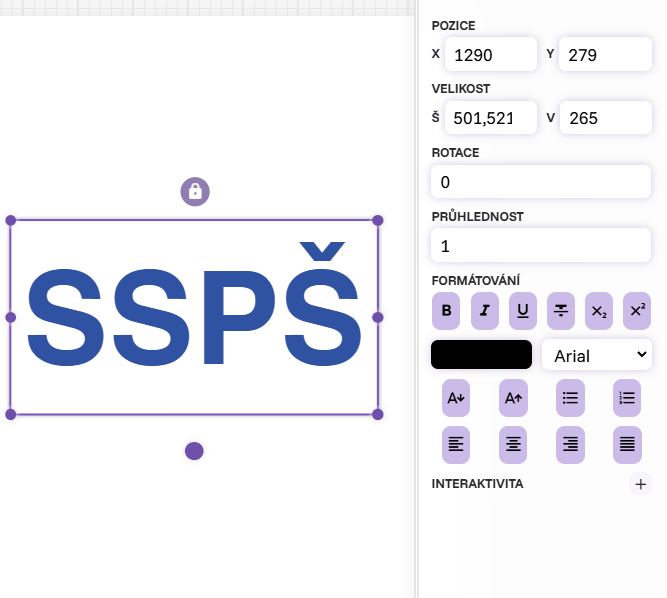
\includegraphics[width=0.8\textwidth]{media/05_realizace/vlastnosti.png}
    \caption{Panel vlastnosti v~editoru pro blok textu}
    \label{fig:realizace/vlastnosti}
\end{figure}

\subsubsection{Historie}

Editor průběžně zaznamenává veškeré důležité události, které se v~jeho prostředí odehrávají. 
Při každé takové události se uloží celý stav editoru, což umožňuje následnou práci s~historií změn. 
Uživatel se může pohybovat zpět nebo vpřed pomocí klasických operací typu \enquote{Zpět} a \enquote{Znovu}. Tento mechanismus využívá princip podobný návrhovému vzoru \emph{memento}~\cite{kerievsky_2004}, kdy se každá změna zaznamenává jako izolovaný snímek stavu editoru.

Velikost uchovávané historie je konfigurovatelná podle preferencí uživatele, aby bylo možné optimalizovat výkon při práci s~rozsáhlými materiály. 
Kromě standardních událostí, které editor sám rozpoznává, existuje i~speciální událost.
Tuto událost mohou vyvolat jiné části systému, například při importu dat nebo externích úpravách, na které není možné se v~editoru běžně zaregistrovat.

\subsubsection{Schránka}

Součástí editoru je vlastní implementace schránky, která umožňuje uživatelům kopírovat a vkládat bloky. 
Tyto operace fungují napříč stránkami jednoho otevřeného dokumentu, ale také mezi různými materiály, které má uživatel současně otevřené. 
Schránka zachovává obsah mezi jednotlivými návštěvami editoru, což zajišťuje plynulost práce i~při opuštění nebo obnově relace.

Kopírování respektuje vnitřní strukturu bloků a umožňuje jejich vkládání bez ztráty informací. 
To je užitečné zejména při vytváření šablon, duplikování opakujících se částí obsahu nebo přenášení obsahu mezi různými snímky.

Uživatel přesto může kopírovat obsah z~jiných částí počítače a vkládat ho například do textových bloků.
Schránka v~aplikace se používá jen tehdy, když uživatel nedělá žádné komplexní akce a kliká na plátno v~editoru -- tedy obyčejná schránka funguje např. uvnitř vstupního pole pro text.

\subsubsection{Nastavení}

Uživatel má možnost upravit široké spektrum nastavení, která ovlivňují chování editoru. 
Kromě základních preferencí lze definovat například maximální velikost historie změn, počet kroků při otáčení objektů nebo způsob provádění transformací.

Editor nabízí několik režimů transformace a různé možnosti chování při zarovnávání či počtu bodů přichytávání při rotaci objektů. 
Díky těmto volbám si může každý uživatel přizpůsobit prostředí svým potřebám -- ať už preferuje jakoukoliv práci.

Všechna nastavení se ukládají do profilu uživatele, takže při každém otevření editoru jsou znovu automaticky načtena.

\subsection{Přehrávač}

Přehrávač sdílí mnoho společných rysů s~editorem, avšak přináší několik klíčových odlišností. 
Stejně jako editor využívá systém bloků a vlastní způsob vykreslování, ale je navržen primárně pro konzumaci a interakci s~výukovým materiálem, nikoli jeho úpravu.

Zásadním rozšířením přehrávače oproti editoru je přidání režimu kreslení. 
Tento režim umožňuje uživateli vybírat barvu, nastavovat tloušťku čáry, úroveň průhlednosti nebo aktivovat stabilizaci tahu. 
K dispozici jsou i~akce jako mazání jednotlivých tahů, skrytí či smazání celé kresby.

Uživatelské rozhraní přehrávače umožňuje přepínat mezi snímky buď pomocí tlačítek, nebo kliknutím na samotné plátno.
Interakce se snímky tak zůstává plynulá a intuitivní. 

Samotné bloky mohou reagovat na uživatelské vstupy díky systému interaktivity a speciálním blokům z~rozšíření.

\subsection{Interaktivita}

Každý blok může mít přiděleno neomezeně mnoho instancí interaktivity, které určují jeho chování při specifických událostech. 
Každá interaktivita definuje událost spuštění interakce a podmínku spuštění.
Všechny další vlastnosti se mění dle vybraných možností.

Události spuštění:
\begin{description}
  \item[CLICK] Aktivace po kliknutí na blok.
  \item[HOVER START] Aktivace při najetí kurzorem.
  \item[HOVER END] Aktivace při odjetí kurzoru.
  \item[SLIDE LOAD] Aktivace při načtení snímku, bez ohledu na blok.
  \item[TIMER] Spuštění po určitém čase, jednorázově nebo opakovaně.
\end{description}


\begin{figure}[ht!]
    \centering
    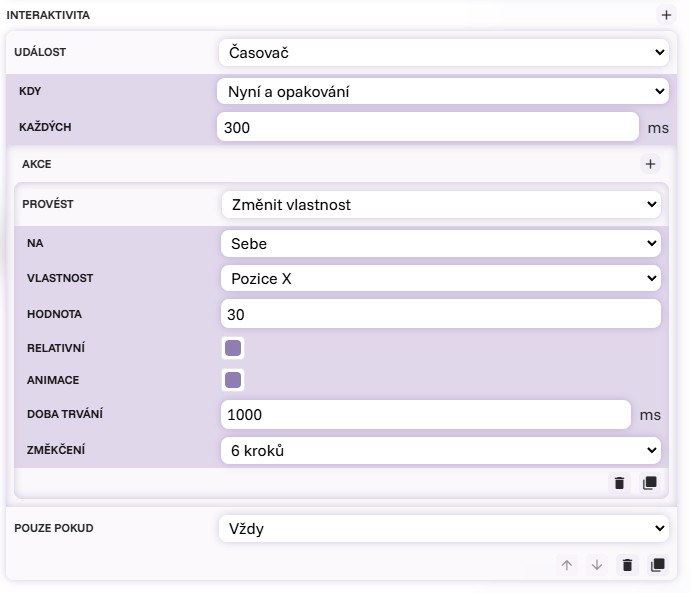
\includegraphics[width=0.8\textwidth]{media/05_realizace/interaktivita.png}
    \caption{Rozhraní interaktivity na bloku v~Editoru}
    \label{fig:interaktivita}
\end{figure}


Podmínky spuštění:
\begin{description}
  \item[ALWAYS] Akce se spustí vždy.
  \item[TIME PASSED] Po uplynutí určitého času od načtení snímku nebo zapnutí celého materiálu.
  \item[VARIABLE] Na základě hodnoty specifické proměnné.
\end{description}

Interaktivita může obsahovat libovolné množství akcí. Mezi základní akce patří:

\begin{description}
  \item[CHANGE PROPERTY] Změní zaregistrovanou vlastnost bloku.
  \item[RESET PROPERTY] Vrátí vlastnost do původního stavu.
  \item[CHANGE SLIDE] Přejde na jiný snímek – konkrétní, relativní, nebo náhodný.
  \item[CHANGE VARIABLE] Upraví hodnotu proměnné.
  \item[OPEN LINK] Otevře externí odkaz.
\end{description}

Akce se mohou vztahovat na konkrétní bloky, všechny bloky na snímku, nebo aktuální blok. 
Systém podporuje interpolaci pro plynulé přechody hodnot a možnost zadávat relativní změny.
Vlastnosti, které lze měnit, si každý blok definuje samostatně pomocí rozhraní v~kódu (viz kód~\ref{code:zapisVlastnostiEditor} a~\ref{code:zapisVlastnostiPrehravac}).

Ukázka nastavené interaktivity na bloku lze vidět na obrázku~\ref{fig:interaktivita}.

Tyto interaktivity jsou zpracovávány přímo přehrávačem a mohou být snadno laděny pomocí ladícího režimu, který zobrazuje stav proměnných. 
Pro jednodušší práci s~interaktivitou byl vytvořen i~speciální blok -- a to interaktivní oblast.
Tento blok umožňuje definovat akce, které nejsou navázané na žádný konkrétní vizuální prvek, ale slouží jako neviditelný spouštěč událostí.

\subsection{Multimédia}

Součástí editoru je možnost vkládat multimediální obsah, zejména obrázky a animované GIF.
Uživatel má k~dispozici dvě základní cesty: buď využije integrované knihovny, nebo nahraje vlastní soubory. 
V obou případech lze multimédia vložit přímo do výukového materiálu jednoduchým kliknutím.

\begin{listing}[ht!]
\caption[Zápis registrace vlastnosti bloku tvaru pro editor]{Zápis registrace vlastnosti bloku tvaru pro editor, \textit{kód zkrácen a modifikován pro přehlednost}}\label{code:zapisVlastnostiEditor}
\begin{minted}{javascript}
public override getInteractivityProperties() {
  return [
    ...super.getInteractivityProperties(),
    {
      label: "Color",
      animate: true,
      relative: false
    }
  ];
}
\end{minted}
\end{listing}



\begin{listing}[ht!]
\caption[Zápis registrace vlastnosti bloku tvaru pro přehrávač]{Zápis registrace vlastnosti bloku tvaru pro přehrávač, \textit{kód zkrácen a modifikován pro přehlednost}}\label{code:zapisVlastnostiPrehravac}
\begin{minted}{javascript}
public override getInteractivityProperties() {
  return [
    ...super.getInteractivityProperties(),
    {
      label: "Color",
      change: (value: string, relative: boolean, ...) => {
        // Validace
        if (animate) {
          // Interpolace podle dalších předaných hodnot.
          // Často využívána funkce requestAnimationFrame
          //    pro plynulé volání změn.
        } else {
          this.color = value;
          this.synchronize();
        }
      },
      // Pro reset vlastnosti
      getBaseValue: () => this.blockBaseValues.color
    }
  ]
}
\end{minted}
\end{listing}

Pro vyhledávání fotografií slouží napojení na fotobanku Pexels. 
Uživatel může zadat libovolný dotaz a zároveň má možnost vybírat z~aktuálně populárních obrázků. 
U animovaných GIF je použita služba Tenor, která je přístupná skrze Google API. 
Vyhledávání zde probíhá na základě klíčových slov nebo výběrem z~předdefinovaných kategorií.

Nahrané soubory se ukládají do uživatelova účtu a lze je použít opakovaně napříč různými výukovými materiály.
V případě většího množství nahraných souborů je procházení optimalizováno pomocí tzv. lazy-loading, což znamená, že se obsah načítá postupně podle potřeby, a nezatěžuje tak prohlížeč ani připojení zbytečnými daty.

Kromě fotobanky a GIF má uživatel možnost vložit jakýkoli externí odkaz na obrázek.
Tento způsob je vhodný zejména tehdy, pokud uživatel nechce daný obrázek ukládat do systému, ale chce jej pouze referovat. 
O způsobu vložení externího odkazu a respektive o~bloku obrázku pojednává detailně sekce~\ref{text:realizace/vytvoreneBloky}.

\subsection{Kolaborace}

Možnost víceuživatelské kolaborace nad jedním výukovým materiálem je jedním ze stěžejních rysů celé platformy.
Bez její existence by bylo možné pracovat na materiálu pouze z~jednoho zařízení, případně by bylo nutné implementovat zamykání souboru a koordinovat přístupy mezi jednotlivými uživateli. 
To by významně omezilo plynulou spolupráci a editaci v~reálném čase.

Cílem bylo umožnit současnou úpravu jednoho materiálu více uživateli. 
Typickým příkladem je práce z~více zařízení jedním uživatelem nebo kooperace více učitelů. 
Tím, že je kolaborace zajištěna přímo na úrovni serveru (viz sekce~\ref{text:realizace/server}), není nutné řešit tradiční formy zamykání dokumentu.

Při zahájení editace materiálu se na serveru příslušný materiál označí jako \enquote{aktivní} a jeho obsah je načten do paměti. 
Od tohoto momentu není změna ihned uložena do databáze, ale uchovává se dočasně a průběžně se ukládá s~využitím techniky \textit{debounce} -- tedy až ve chvíli, kdy se tři sekundy nic nemění. 
V případě dlouhodobé editace se změny ukládají nejpozději po třiceti sekundách.

Editace probíhá ve speciální místnosti (\textit{material editor room}), do které se mohou připojit všichni uživatelé s~přístupem k~danému materiálu. 
Server v~této místnosti sleduje aktivitu jednotlivých účastníků -- na kterém snímku se nacházejí, jaké bloky mají označené, jejich jméno a barvu. 
Pouze majitel daného materiálu může nastavit, kteří uživatelé mají k~editaci materiálu přístup.

Složité by bylo synchronizovat úpravy jednoho bloku více lidmi současně.
Z tohoto důvodu je na úrovni klienta i~serveru zaveden mechanismus pro zamykání jednotlivých bloků.
V jeden moment může daný blok upravovat pouze jeden uživatel.

Při každé změně -- ať už jde o~přepnutí snímku, označení bloku nebo jeho úpravu -- klient informuje server. 
Server změnu přepošle všem ostatním připojeným účastníkům, čímž je zajištěna konzistence mezi jednotlivými instancemi editoru.
V materiálu u~klienta je v~UI vidět, kdo je k~materiálu připojen, jak se jmenuje a na jakém snímku se aktuálně nachází.
Na daném snímku se poté vykresluje speciální obdélník okolo bloků, které má označené (a které tedy nelze označovat).
Na obrázku~\ref{fig:realizace/kolaborace} lze vidět takto označený blok a seznam účastníků editování.



\begin{figure}[ht!]
    \centering
    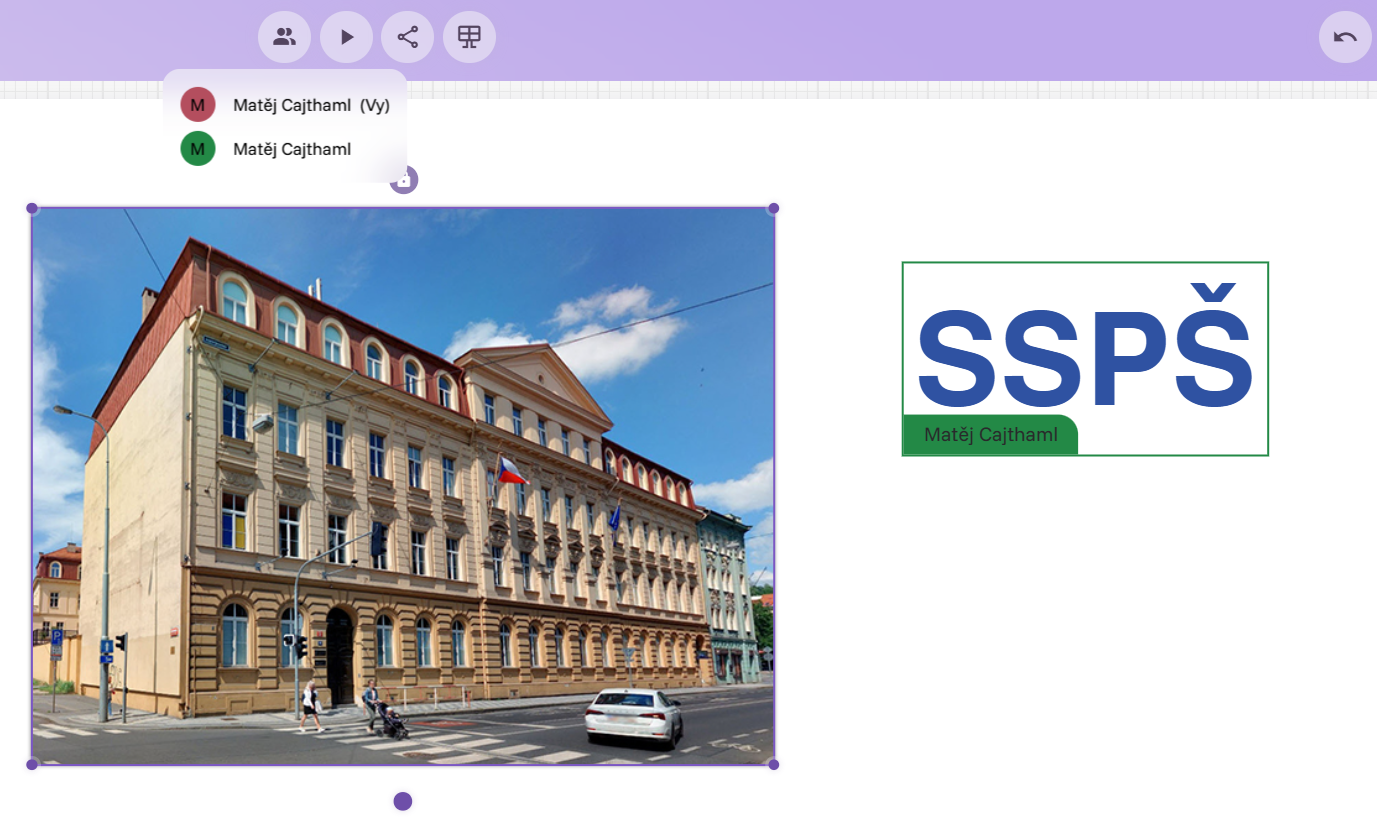
\includegraphics[width=0.8\textwidth]{media/05_realizace/kolaborace.png}
    \caption{Kolaborace v~editoru, označený blok jiným účastníkem a seznam účastníků}
    \label{fig:realizace/kolaborace}
\end{figure}


Server neplní pouze roli zprostředkovatele komunikace. 
Zajišťuje také generování náhledových snímků, správu práv a samotné ukládání dat.
Náhledové snímky se generují pomocí knihovny \texttt{puppeteer} na straně serveru. 
Server v~takovém případě spustí virtuální prohlížeč a kontaktuje speciální stránku na klientovi, která po ověření vykreslí požadovaný snímek bez uživatelského rozhraní, a prohlížeč tuto stránku zachytí. 
Tento vykreslený náhled je poté odeslán zpět a uložen do databáze. 
Výsledkem je velmi přesná vizualizace reálného vzhledu snímku bez závislosti na rozšířeních nebo výkonu zařízení klienta.
Stejně jako u~ukládání probíhá generování náhledů pomocí \textit{debounce} se stejnými časovými limity.
Pro bezpečnost musel být vytvořen systém ochrany neveřejných materiálů, a proto tento virtuální prohlížeč používá svůj systém autorizace k~materiálům.

Nad rámec synchronizace samotného obsahu se mezi klienty přenášejí také další informace o~materiálu -- jeho název, nastavení sdílení nebo vlastnosti přehrávání.
Synchronizují se i~případná rozšíření a další metadata, čímž se zajišťuje, že všichni účastníci mají vždy aktuální stav.

\subsection{Prezentování}


Režim prezentování je klíčovou součástí přehrávače. 
Po jeho spuštění se aplikace nachází vždy v~základním režimu prezentace. 
Tento režim je navržen tak, aby umožnil plynulou vizualizaci výukového materiálu, ať už v~rámci výkladu před třídou, nebo při sdílené distanční výuce.

V editoru lze upravit několik parametrů, které ovlivňují chování přehrávače.
Prvním z~nich je způsob průchodu snímky -- prezentaci lze nastavit tak, aby probíhala automaticky s~časovačem, ručně klikáním, nebo aby byla ovládána výhradně interaktivními prvky.
Další důležitou možností je volba režimu zobrazení.
Snímky lze buď rozprostřít na celou stránku bez možnosti manipulace, nebo ponechat uživateli kontrolu nad pohybem v~rámci plátna (včetně například přiblížení).

Po přechodu do takzvaného \enquote{sledovacího módu} prezentace se chování aplikace změní. 
Prezentující získá jedinečný odkaz, QR kód a textový kód, které může sdílet s~publikem. 
Připojení účastníci potom sledují prezentaci v~synchronizovaném režimu. 
Nemají možnost samostatného pohybu mezi snímky ani úprav obsahu. 
Interagují výhradně skrze interaktivní bloky, které byly do prezentace vloženy v~editoru.

Přehrávač zajišťuje, aby byl aktuální snímek synchronizovaný mezi všemi sledujícími.
Rovněž je synchronizována i~funkce kreslení, kterou může prezentující využít k~doplňování výkladu během prezentace.

Tento režim prezentování je připraven na použití vzdálené komunikace (viz sekce~\ref{text:realizace/vzdalenaKomunikace}).
Díky tomu lze rozšířit výuku o~plně interaktivní prvky, jako je chat, hlasování, nebo různé typy kvízů. 
To zajišťuje, že i~při pasivním sledování prezentace mohou studenti aktivně reagovat a zapojit se do výukového procesu.

Sledování je implementováno podobně jako kolaborace v~editoru, tedy, že existuje speciální místnost, kterou avšak tentokrát tvoří uživatel, který sledování započne.

\subsection{Importování a exportování}

Přestože jsou výukové materiály na platformě koncipovány jako interaktivní, existují případy, kdy je potřeba je převést do statické podoby.
Typicky jde například o~tisk, archivaci nebo tvorbu plakátu. 
Zároveň je důležité, aby měl uživatel možnost uchovávat lokální zálohy materiálů, a tím zvýšit bezpečnost dat mimo samotný server.

Systém proto podporuje jak import, tak export materiálů. 
Architektura je rozdělena mezi klienta a server. 
Import zajišťuje klientská část, která ze zadaného vstupu vytvoří nový materiál včetně odpovídajících bloků. 
Export naopak probíhá na serveru.

Při exportu odešle klient požadavek na konkrétní formát, aktuálně podporované jsou JSON a PDF. 
Export do JSON vrací kompletní strukturu materiálu, respektive jednotlivých snímků, včetně všech vlastností. 
Tento formát je vhodný pro zálohování nebo pozdější import. 
Export do PDF funguje tak, že server pomocí nástroje \texttt{puppeteer} vykreslí každý snímek zvlášť jako náhled. 
Výsledkem je soubor obsahující jednotlivé stránky, které reflektují vzhled snímků tak, jak je vidí uživatel.
Jelikož mohou mít jednotlivé snímky odlišné rozměry, je nezbytné generovat je po jednom a teprve následně spojit do jednoho PDF dokumentu.

Import podporuje klient ze dvou formátů: JSON a Markdown. 
Při importu JSON dojde ke znovuvytvoření materiálu přesně podle předchozí struktury. 
Markdown je zpracován pomocí knihovny \texttt{marked}, která na klientovi vrací stromovou reprezentaci dokumentu. 
Klient následně přečte jednotlivé nadpisy a obsahové bloky mezi nimi a rozdělí je do odpovídajících snímků. 
První nadpis se použije jako název materiálu a titulní strana.

Markdown import podporuje běžné textové struktury jako nadpisy, tučný a kurzívní text, odkazy nebo seznamy. 
Díky tomu je možné rychle vytvořit základní kostru prezentace bez nutnosti ručního zadávání každého bloku.

\section{Rozšíření}

Platforma umožňuje přidávat nové funkcionality pomocí tzv. pluginů. 
Každý plugin má své jedinečné jméno a krátký popis, který vysvětluje jeho účel a hlavní funkce. 
Plugin může existovat v~několika verzích, přičemž každá verze obsahuje manifest, kód pluginu a případně specifický kód pro editor.
Manifest obsahuje informace o~tom, pro jakou verzi aplikace bylo rozšíření napsáno a různá další data, jako je například nastavení přístupu k~doménám či jiným pravomocem.

Manifest dále obsahuje verzi pluginu vůči celému systému.
To dovoluje vytvořit převratné změny v~API, a dovolí to jasně diferencovat to, pro jakou verzi je dané rozšíření napsáno, a v~případě, že se verze API změní, tak všechny pluginy bez této verze přestanou fungovat.

Verzování bloků si pak každé rozšíření řeší samo.
Do bloků si může ukládat verze a pokud nastane změna, tak si je sám může překonvertovat při zapnutí.

Uživatelé, resp. vývojáři, mohou pluginy jednoduše přidávat přímo v~aplikaci, pokud jsou přihlášeni, a také mají možnost nahrávat nové verze stávajících pluginů. 
% K~zajištění bezpečnosti a kvality je implementován systém schvalování, který ověřuje, zda pluginy splňují stanovená kritéria před jejich zveřejněním.

Rozšíření a jejich API jsou dokumentována v~dokumentaci platformy.
Pro lepší vývoj byly vytvořeny typy, které lze používat i~v~programování v~jazyce JS.
Ty napovídají v~moderních vývojových prostředích vývojářům rozšíření s~tím, co mohou za věci ve vytvořeném API používat.

Ukázku typů lze najít v~kódu~\ref{code:realizace/typy}, celé typy lze najít v~kódové příloze v~souboru \verb|/platform/plugins/types.d.ts|.


\begin{listing}[ht!]
\caption[Část vytvořených typů pro platformu rozšíření]{Část vytvořených typů pro platformu rozšíření, \textit{kód zkrácen a modifikován pro přehlednost}}\label{code:realizace/typy}
\begin{minted}{typescript}
interface ApiPlayer {
    /**
     * Returns all blocks in the player slide.
     * @returns An array of blocks in the player slide.
     */
    getBlocks(): PlayerBlock[];
    /**
     * Removes a block from the player. The block will be removed 
     * from the player and the player will be updated.
     * If the block is not found, nothing happens.
     * @param id The ID of the block to remove.
     */
    removeBlock(id: string): void;
    /**
     * Add a new block to the player. The supplied data has to be
     * in the correct format for the block type.
     * @param block The block data to add to the player.
     * @returns The ID of the newly added block.
     */
    addBlock(block: CreatePlayerBlock): string;
    // ...
}
\end{minted}
\end{listing}

\subsection{Spouštění kódu}

Spouštění kódu pluginů probíhá bezpečně v~prostředí QuickJS, jak je uvedeno v~návrhu v~sekci~\ref{text:navrh/plugins}. 
Kód pluginů má omezený přístup pouze k~API editoru a obsahu stránky prostřednictvím definovaného rozhraní. 
Přístup k~jakýmkoliv dalším zdrojům mimo tento rámec není možný ze zabezpečení knihovny QuickJS a jejich systému.

\subsection{Přístup k~API}

Platforma poskytuje pluginům jasně definované globální API zahrnující funkce, jako je:

\begin{description}
    \item[fetch] která dovoluje volat požadavky přímo jako stránka editoru (tj. s~CORS) na povolených doménách z~manifestu.
    \item[cache] která dovoluje rozšíření si pamatovat věci skrz spuštění.
    \item[plugin] která dovoluje vědět, kdo je aktuálním spouštěčem skriptu.
    \item[language] která dovoluje zjistit, jaký jazyk je aktuálně vybrán.
    \item[log] která dovoluje vypisovat věci do konzole pro lepší vývoj.
\end{description}

Dále mohou pluginy využívat API jednotlivých bloků, které umožňuje přístup k~jejich vlastnostem a metodám.
Například se jedná o~funkce jako manipulaci bloku, změnu obsahu a další.

Dále rozšíření, podle toho, kde jsou spuštěny, dovolují přistupovat ke konkrétním API přehrávače či editoru.

Editor API nabízí možnost číst bloky, přidávat nové bloky a nastavovat různé režimy a velikosti pracovního plátna. 
Podobně funguje i~Player API, které rovněž umožňuje čtení a přidávání bloků spolu s~nastavením režimů, velikostí a aktuálního snímku.

\subsection{Zachycení se k~událostem}

Každému rozšíření začíná životní cyklus voláním globální exportované funkce se jménem \texttt{initEditor} ve spuštění v~editoru, případně \texttt{initPlayer} v~přehrávači.
V této metodě může rozšíření spouštět řadu věcí a již interagovat s~API.
Základně v~této metodě se budou programátoři rozšíření připojovat zejména k~událostem, které způsobí to, že když daná událost nastane, tak se zavolá i~příslušná funkce k~této události od tohoto rozšíření. 
Ukázka zachycení k~události a prvotního načtení je vyobrazena v~kódu~\ref{code:registraceUdalosti}.

Pro editor a přehrávač (ne nutně pro oba) existují následující události:

\begin{description}
    \item[pluginBlockRender] Tato událost se volá tehdy, když je blok typu \texttt{plugin} vykreslován. Událost se volá jen pro rozšíření, které blok vlastní. Volá se sporadicky, zpravidla jenom při prvotním načtení editoru či přehrávače. 
    \item[panelRegister] Tato událost se volá tehdy, když je uživatelské rozhraní připraveno získat informace o~tom, jaký plugin požaduje jaké panely v~rozhraní editoru. Na událost musí funkce vracet HTML, které se vykreslí v~iframe. O~bezpečnosti této metody viz sekci~\ref{text:vykreslovani}.
    \item[panelMessage] Událost se volá tehdy, když panel přiřazen tomuto rozšíření chce předat zprávu rozšíření. Předávaná data jsou vždy v~textovém řetězci.
    \item[pluginBlockMessage] Tuto událost volá konkrétní blok v~editoru či přehrávači právě tehdy, když chce předat zprávu rozšíření. Předávaná data jsou taktéž v~textovém řetězci.
    \item[pluginBlockPropertyChange] Tato událost se volá tehdy, když v~uživatelském rozhraní editoru uživatel změní konkrétnímu bloku vlastnost. Rozšíření pomocí parametrů ví, jaká konkrétní vlastnost se změnila a na jakém bloku.
    \item[pluginRemoteMessage] Tato událost se volá tehdy, když blok vlastněný tímto rozšířením obdrží zprávu od vzdáleného bloku stejné instance. Více se o~vzdálené komunikaci zmiňuji v~sekci~\ref{text:realizace/vzdalenaKomunikace}. 
\end{description}


\subsection{Vykreslované bloky}

Platforma poskytuje pluginům možnost definovat a vykreslovat vlastní bloky, které jsou součástí vizuální reprezentace materiálů.
Tyto bloky mohou sloužit k~rozšíření funkcionality uživatelského rozhraní, například formou interaktivních ovládacích prvků, vizualizací nebo jako prostředek pro zobrazení dynamického obsahu.

Každý blok je definován prostřednictvím příslušného pluginu, který specifikuje jeho identifikátor, vykreslovací logiku a případné konfigurační parametry. 
Vykreslování samotného bloku pak zajišťuje platforma voláním odpovídající vykreslovací funkce, kterou plugin poskytuje. 

Bloky mohou být navrženy tak, aby podporovaly obousměrnou komunikaci s~pluginem, který je spravuje. 
To znamená, že blok může přijímat data a instrukce ze svého pluginu a současně do něj zasílat zpětné informace, typicky ve formě událostí nebo změn stavu. 
Tento princip umožňuje tvorbu dynamických a interaktivních komponent, které se mohou automaticky aktualizovat na základě vstupu od uživatele nebo změn v~aplikační logice.

Překreslování bloků je platformou optimalizováno s~cílem minimalizovat výkonnostní dopad. 
Nedochází k~němu při každé drobné změně, ale spíše jen ve chvílích, kdy je to nezbytné pro zachování konzistence zobrazeného obsahu~-- tedy zejména při inicializaci nebo po zásadní změně konfigurace.

Definice a registrace vlastních bloků probíhá prostřednictvím rozhraní poskytovaného platformou, přičemž vývojář pluginu má plnou kontrolu nad tím, jaký obsah blok zobrazuje a jak reaguje na různé typy vstupů. 
V dokumentaci systému jsou uvedeny konkrétní příklady definice bloků, včetně popisu příslušných metod a událostí.


\subsection{Panel}

Pluginy v~systému mají možnost registrovat vlastní uživatelské panely, které se vykreslují jednorázově jako součást rozhraní aplikace. 
Tyto panely poskytují prostor pro interaktivní prvky, sloužící primárně k~řízení chování pluginu a jeho propojení s~dalšími částmi systému, zejména s~vykreslovanými bloky.

Panel je typicky využíván k~implementaci rozhraní pro konfiguraci, správu uživatelských vstupů nebo jako nástroj pro zprostředkování výměny dat mezi jednotlivými komponentami pluginu. 
Běžným příkladem je vytvoření formuláře pro zadávání parametrů nového bloku, editace existujících prvků či zobrazení informací relevantních pro daný plugin.

Z technického hlediska je panel realizován jako samostatný Iframe, jehož obsah je řízen pluginem. 
Komunikace mezi tímto panelem a ostatními částmi systému (např. hlavní aplikací nebo vykreslenými bloky) probíhá prostřednictvím rozhraní postaveného na standardu \texttt{postMessage}, které je součástí webového API moderních prohlížečů. 
To umožňuje bezpečnou a efektivní výměnu zpráv mezi oddělenými kontexty, přičemž každá zpráva je jednoznačně identifikována a zpracována příslušnou částí systému.

V rámci vývoje pluginu je nezbytné definovat způsob, jakým panel odesílá a přijímá zprávy. 
Aplikace poskytuje vlastní API, které nad rámec běžného \texttt{postMessage} rozšiřuje funkcionalitu o~specifické události, zpracování chyb nebo obsluhu odpovědí. 
Ukázka takové komunikace je uvedena v~kódu~\ref{code:registraceUdalosti}, kde je demonstrována registrace obsluhy zpráv přicházejících z~panelu.

\begin{listing}[ht!]
\caption[Ukázkový zápis rozšíření a registrace na událost]{Ukázkový zápis rozšíření a registrace na událost, \textit{kód zkrácen a modifikován pro přehlednost}}\label{code:registraceUdalosti}
\begin{minted}{javascript}
export const onPanelMessage = (message) => {
  if (message !== "clicked") return;

  // Zde se provádí akce po kliknutí na tlačítko
  api.editor.addBlock({
    type: "text",
    // ... další vlastnosti bloku
  });
}

export const initEditor = function () {
  api.editor.on("panelMessage", onPanelMessage);
  api.editor.on("panelRegister", () => {
    // Zavolání např. api.fetch
    return `<button>Click me</button>
      <script>
      document.querySelector("button").addEventListener("click", 
        () => {
            window.parent.postMessage({
                target: "script", message: "clicked"
            }, "*");
        });
      </script>`;
  });
}
\end{minted}
\end{listing}

Z pohledu uživatele je panel obvykle přístupný prostřednictvím uživatelského rozhraní materiálu v~podobě postranní navigace. 
Její obsah je zcela v~kompetenci pluginu, což umožňuje značnou míru přizpůsobení vzhledu i~chování dle konkrétních potřeb.

Ukázka panelu z~ukázkového pluginu lze vidět na obrázku~\ref{fig:realizace/panel}.




\begin{figure}[ht!]
    \centering
    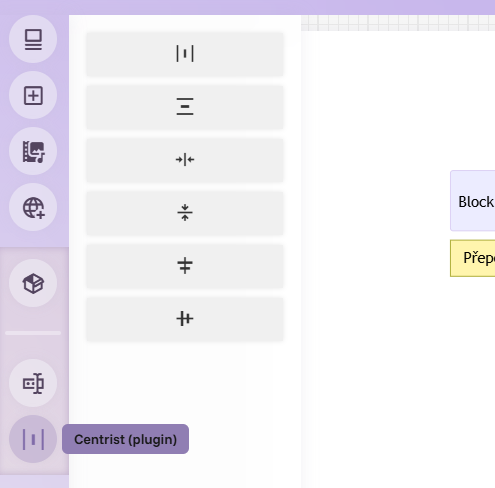
\includegraphics[width=0.8\textwidth]{media/05_realizace/panel.png}
    \caption{Zaregistrovaný panel rozšíření v~aplikaci}
    \label{fig:realizace/panel}
\end{figure}

\subsection{Vzdálená komunikace}\label{text:realizace/vzdalenaKomunikace}

Pro možnost tvořit interaktivní materiály jsem v~práci vytvořil systém vzdálené komunikace.
Vzdálená komunikace v~tomto případě znamená komunikaci v~reálném čase mezi bloky.
Tento systém dovoluje výměnu zpráv mezi jedním blokem v~různých instancích přehrávače na různých počítačích.

Pokud přednášející či učitel zapne materiál ke sledování, každý blok může přijímat testové zprávy.
Aplikace se v~tomto případě chová jako zprostředkovatel zpráv a určuje, kdo komu může odeslat zprávy.
Každý blok si validuje zprávy sám.

Jediné dvě možné cesty komunikace jsou:

\begin{itemize}
    \item Od prezentujícího všem sledujícím.
    \item Od sledujícího prezentujícímu.
\end{itemize}

Tento systém dovoluje různorodost bloků, které závisí na prezentujícím.
Tyto směry jsem navrhl tak, že blok prezentujícího slouží jako hlavní správce komunikace.
Tento blok se může rozhodnout, zda zprávy někomu zašle.
Systém mu předá zprávu a identifikátor vzdáleného propojení v~protokolu WebSockets.
Tento systém dovoluje řadu způsobů komunikace, níže uvádím dle mého názoru dva nejdůležitější.

\begin{description}
    \item[Přeposílání] -- kde blok prezentujícího okamžitě odešle zprávu po obdržení všem připojeným sledujícím. Způsob lze použít např. na okamžité odpovědi, chat a další.
    \item[Udržování] -- kde blok prezentujícího obdržené zprávy ponechává a odešle je najednou např. po časovém limitu. Tento způsob lze použít například na kvízy či na \enquote{čas pro přemýšlení}.
\end{description}

Komunikaci mohou používat všechny bloky a to dokonce i~bloky vytvořené pro rozšíření.
Místo toho, aby komunikaci spravoval blok, spravuje ho pro tyto bloky rozšíření, které se může zachytit na událost \verb|pluginRemoteMessage|.
Rozšíření tuto zprávu může zpracovat a odeslat ostatním podle svých možností. 
Znovu je možné použít komunikaci s~blokem pro vykreslení obsahu uvnitř bloku.
Tato komunikace je poté složitější a ukázka toho, jak vypadá, je na obrázku~\ref{fig:realizace/vzdalenaKomunikace}.

\begin{figure}[ht!]
    \centering
    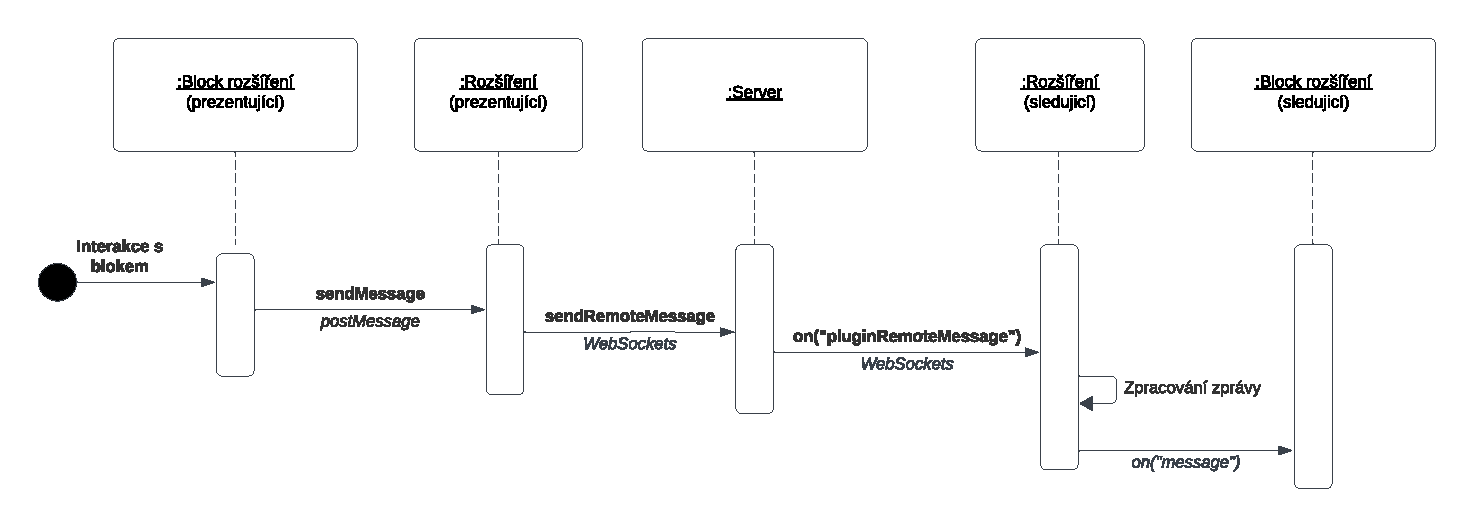
\includegraphics[width=1\textwidth]{media/05_realizace/vzdalenaKomunikace.pdf}
    \caption{Diagram vzdálené komunikace bloků}\label{fig:realizace/vzdalenaKomunikace}
\end{figure}


\section{Hlavní webová stránka}\label{text:realizace/hlavniStranka}


Hlavní webová stránka byla vytvořena za účelem propagace aplikace.
Celý projekt a aplikace nese název \textbf{Materalist}.
Název vznikl spojením slov \textit{Material} a \textit{Specialist}, čímž odkazuje na zaměření aplikace na práci s~různými specializovanými materiály.
Slouží jako výchozí bod pro návštěvníky, kteří se chtějí dozvědět více o~aplikaci, jejích funkcích a možnostech využití. 
Stránka umožňuje přesměrování na samotnou aplikaci, přístup k~dokumentaci a obsahuje přehled funkcionalit.

\begin{figure}[ht!]
    \centering
    
\includegraphics[width=0.3\textwidth]{media/05_realizace/logo.png}
    \caption{Logo aplikace Materalist}
    \label{fig:logo}
\end{figure}

Důležitou součástí webové prezentace je porovnání s~ostatními aplikacemi v~daných oblastech. 
To pomáhá uživatelům lépe pochopit výhody a jedinečné vlastnosti aplikace. 
Kromě toho webová stránka představuje dostupné pluginy, které rozšiřují základní funkcionalitu aplikace.

Design webové stránky vychází a inspiruje se z~vizuálního stylu samotné aplikace (viz sekce~\ref{text:realizace/klient}). 
Stránka je responzivní a optimalizovaná pro různé typy zařízení.

Pro sjednocení vizuální identity bylo navrženo logo aplikace (viz obrázek~\ref{fig:logo}), které symbolizuje kombinaci plátna a písmene \enquote{M}, což reflektuje jak materiálový aspekt, tak kreativní přístup k~tvorbě obsahu.

Hlavní webová stránka byla tvořena taktéž ve webovém frameworku Vue, ze stejných důvodů jako hlavní aplikace.
Hlavním konceptem je velká jednostránková webová stránka, která obsahuje všechny důležité informace a odkazuje na dokumentaci a samostatnou aplikaci.
Stránka obsahuje zmíněné funkcionality, popis toho, co aplikace je, a taktéž seznam ukázkových materiálů, které může kdokoliv přidat.

Tato stránka obsahuje taktéž právní informace, a to podmínky používání a informace o~ochraně osobních údajů.


\section{Dokumentace}

Pro dokumentaci projektu byl použit nástroj Docusaurus. 
Zvolil jsem ho kvůli podpoře psaní ve formátu Markdown, jednoduché správě obsahu a možnosti rychlého nasazení. 
Dokumentace je strukturovaná do dvou hlavních částí: použití a rozšiřování.

První část, zaměřená na použití, slouží jako uživatelská příručka k~webové aplikaci. 
Obsahuje přehled uživatelského rozhraní, popis jednotlivých sekcí aplikace a vysvětlení dostupných funkcí. 

Druhá část je určena vývojářům, kteří chtějí projekt rozšiřovat. 
Pokrývá možnosti úprav kódu i~práci s~pluginy. 
Podrobně popisuje postup při lokální instalaci, strukturu a API dostupných pluginů i~způsob, jakým lze vytvářet vlastní. 
Vývoj pluginů je vysvětlen krok za krokem, včetně propojení s~existujícími typy z~TS pro jejich tvorbu.

Celý obsah je psaný v~angličtině, aby byl přístupný širší komunitě. 
Text je doplněn odkazy mezi jednotlivými stránkami, což umožňuje snadnou orientaci.

\section{Sestavení a nasazení aplikace}\label{text:realizace/nasazeni}

V této sekci popisuji, jak lze výslednou aplikaci sestavit a jak jsem ji nasadil do produkce.
Taktéž popisuji, jak lze nadále jednoduše vyvíjet aplikaci pomocí jednoduchého nasazení. 

\subsection{Sestavení}

Každou část aplikace lze sestavit samostatně pomocí sestavovacích skriptů \verb|build| v~\verb|npm| projektu.
Takové sestavení však potřebuje správné nastavení proměnných systémů, aby došlo ke správnému propojení nahraných aplikací.
O celkovém sestavení si lze přečíst v~dokumentaci aplikace.

Výsledné části lze poté hostovat jako statické stránky, tedy se jedná o~projekty hlavní stránky, aplikace, dokumentace.
Výslednou část serveru je nutné hostovat jako Node.js aplikaci na serveru.
K tomu je potřeba mít nasazenou databázi typu MongoDB.

Obecně tento způsob není vhodný pro jednoduché nasazení a vyžadoval by velké zkušenosti jak s~aplikací, tak s~propojením jednotlivých částí. 

\subsection{Nasazení pomocí služby Docker}

Celý systém je kontejnerizovaný pomocí služby Docker.
V kořenovém adresáři repozitáře se nachází soubor \texttt{docker-compose.yml}, který zajišťuje spuštění všech částí aplikace. 
Každá komponenta má svůj vlastní \texttt{Dockerfile}, ve kterém je definováno její specifické prostředí a závislosti.

Pro sjednocení konfigurace je využit globální soubor \texttt{.env}, ve kterém jsou definované klíčové proměnné. 
Tento soubor slouží jako centrální místo pro předávání informací do jednotlivých částí systému. 
Služba Docker Compose tyto proměnné předává dál a zároveň přidává vlastní proměnné pro vzájemné propojení mezi kontejnery. 
Tímto způsobem je možné jednoduše konfigurovat běh celého systému z~jednoho místa.

\subsection{Nasazení na produkci}

Na produkční nasazení jsem zaregistroval vlastní doménu \href{https://materalist.com}{materalist.com}, na které běží všechny části systému.  
Níže jsou uvedeny odkazy na nahrané části aplikace.

\begin{description}
    \item[Hlavní stránka] \href{https://materalist.com}{https://materalist.com}
    \item[Dokumentace] \href{https://docs.materalist.com}{https://docs.materalist.com}
    \item[Aplikace] \href{https://app.materalist.com}{https://app.materalist.com}
    \item[Server] \href{https://api.materalist.com}{https://api.materalist.com}
\end{description}

Výsledná aplikace, respektive její uživatelské rozhraní, je k~zobrazení taktéž na obrázcích v~příloze~\ref{appendix:uzivatelskeRozhrani} včetně ukázky hlavní stránky a dokumentace.

DNS záznamy spravuji pomocí služby Cloudflare, která zároveň zajišťuje automatické vydávání certifikátů pro HTTPS a end-to-end šifrování. 
Veškerý provoz tak probíhá šifrovaně a zabezpečeně.

Celý systém běží na vlastním serveru. 
Na serveru je nastavená reverzní proxy pro připojení různých domén na jednom portu.
Pro nasazení využívám opět Docker Compose ve stejné struktuře jako ve vývojovém prostředí.
Nové verze se nahrávají automaticky pomocí GitLab Actions. 
K nasazení používám nástroj \texttt{rsync} přes SSH. 
Sestavení obrazů probíhá až na serveru, což minimalizuje přenos dat a zjednodušuje ladění. 
Nasazení je navrženo tak, aby probíhalo bez výpadků. 
Citlivé proměnné jsou v~repozitáři maskované a server k~nim přistupuje přes zabezpečené prostředí.

\subsection{Vývoj}

Vývojové prostředí využívá upravené varianty stejných souborů \texttt{Dockerfile} a \texttt{docker-compose.yml} z~nasazení na produkci. 
Pro každou část systému existuje vlastní vývojová konfigurace, která umožňuje rychlé spuštění.

Na rozdíl od produkce se při vývoji nepoužívá \texttt{volume} pro mount celého projektu, ale jen pro adresáře mimo \texttt{node\_modules}, kontejner pak otevře projekt v~módu \texttt{live-reload}.
Vývojáři tak mohou spustit celý systém jedním příkazem, bez nutnosti dalších úprav, a vyvíjet platformu.

\section{Vytvořené bloky}\label{text:realizace/vytvoreneBloky}

Pro účely demonstrace schopností platformy a testování její flexibility byla implementována základní sada bloků.
Tyto bloky jsou přímo dostupné v~rámci editoru a byly navrženy tak, aby pokrývaly široké spektrum typických potřeb při tvorbě vzdělávacích materiálů. 
Bloky reagují na nastavení v~panelu vlastností a mění se podle toho, jaké možnosti autor obsahu zvolí. 
Některé bloky se po kliknutí přepnou do editačního režimu a umožní přímou úpravu svého obsahu, například textu nebo kódu. 

\subsection{Text}

Textový blok slouží pro vkládání formátovaného textu. 
Uživatel může upravit styl písma, jeho velikost a barvu, použít tučné, kurzívní, podtržené nebo přeškrtnuté písmo. 
Dále lze nastavit zarovnání textu (vlevo, vpravo, na střed i~do bloku), font, horní a dolní index a také vytvářet seznamy. 

Po kliknutí na blok se aktivuje textový editor, ve kterém lze přímo označovat a upravovat text. 
Veškeré změny jsou zároveň reflektovány v~panelu vlastností, odkud lze pohodlně ovlivnit celkové formátování. 
Vnitřně se text ukládá jako HTML, ale pro vykreslení se používá knihovna \texttt{sanitize-html}, která omezuje vykreslení jen na bezpečné a povolené značky a atributy.

\subsection{Obrázek}

Obrázkový blok umožňuje vkládání obrázků pomocí URL adresy. 
Je využíván především v~obsahových menu, kde lze vybírat z~fotobank, GIF nebo vlastních multimédií. 
Pro přesnější práci s~obrázky je k~dispozici funkce pro uzamčení poměru stran. 
Pokud je aktivní, obrázek se při změně velikosti bloku přizpůsobuje původnímu poměru. 

V opačném případě dochází k~tzv. překrytí -- obrázek si ponechává původní rozměry a v~případě menšího prostoru se jeho část ořízne.
Pokud se obrázek nepodaří načíst, editor zobrazí varování, přehrávač však zůstává tichý.

\subsection{Interaktivní oblast}

Tento blok je viditelný pouze v~editoru, nikoli v~přehrávači.
Slouží jako neviditelná vrstva, která umožňuje překrýt více prvků a zajistit, že se jejich interaktivita nebude vzájemně ovlivňovat.
Jde o~užitečný nástroj především pro složitější kompozice.

\subsection{Diagram}

Pro tvorbu různých typů diagramů je využita knihovna \texttt{mermaid}. 
Umožňuje kreslit UML diagramy, grafy a další pomocné vizualizace. 
Uživatel může po kliknutí na blok upravit zdrojový kód diagramu. 
Mimo editační režim se automaticky vykresluje výsledný diagram.

Pokud kód obsahuje chybu, editor zobrazí varování a místo náhledu diagramu vykreslí hlášení.
V přehrávači se chybové bloky neobjevují. 
Vzhledem ke známým bezpečnostním rizikům (XSS zranitelnosti) a komplikacím při interakci byla implementace řešena pomocí Iframe.

\subsection{Iframe okno}

Iframe blok slouží pro pokročilé uživatele, kteří chtějí do editoru vložit vlastní HTML, CSS nebo JavaScript. 
Blok umožňuje spustit libovolný kód v~izolovaném prostředí a zobrazit jeho výsledek přímo v~editoru.

Editace probíhá kliknutím na blok, kdy se otevře rozhraní pro úpravu kódu. 
Výstup se mimo editační režim vykreslí automaticky. 
Kvůli bezpečnostním rizikům a nemožnosti opustit Iframe z~vnitřního prostředí je nutné tento způsob používat obezřetně, viz sekce~\ref{text:anaylza/spousteniNeduveryhodnehoKodu}.

\subsection{Tvar}

Tvarové bloky poskytují jednoduchý způsob, jak do materiálu přidat vizuální strukturu. 
Obsahují základní předdefinované tvary jako obdélník, hvězda nebo elipsa. Uživatel může upravit barvu tvaru.

Některé tvary se dokážou přizpůsobit velikosti bloku -- typickým příkladem je šipka, která natahuje svůj střed dle aktuálních rozměrů.
Tyto bloky slouží jako doplňkový vizuální prvek, který zvyšuje čitelnost a srozumitelnost obsahu.

\subsection{Chat}

Blok chatu dovoluje komunikaci při době prezentování materiálu mezi sledujícími.
Blok používá vzdálenou komunikaci (viz sekce~\ref{text:realizace/vzdalenaKomunikace}).
Prezentujícímu se ukazuje box se zprávami a může se do konverzace zapojit.
Jako prezentující taktéž můžete posílání zpráv pozastavit.

Sledující si v~chatu může vybrat jméno, nebo bez něj bude používat identifikátor připojení WebSocket.

\subsection{\LaTeX}

Blok dovoluje zápis \LaTeX rovnic a jiných matematických výrazů.
Tento blok je ideální pro prezentace zaměřené na matematiku, fyziku, informatiku nebo jiné technické obory, kde je potřeba přesně vyjádřit symbolické a matematické výrazy.
Pro vykreslení je používána knihovna KaTeX.

\subsection{Kód}

Kódový blok dovoluje vkládat kód přímo do prezentace s~tím, že bude automaticky obarvovat syntaxi klíčových slov a jiných jazykových konstrukcí.
Blok taktéž dovoluje zapnout číslování jednotlivých řádků pro jednodušší ukazování během prezentace.

Do budoucna by bylo vhodné tento blok více rozšířit a dovolit například animace zvýraznění jednotlivých řádků či různé přechody mezi jednotlivými zápisy.

\section{Vytvořené rozšíření}\label{text:realizace/vytvoreneRozsireni}

Součástí návrhu platformy byla i~možnost komunitního rozšiřování funkcionality prostřednictvím pluginů. 
Tato sekce představuje několik ukázkových rozšíření, která byla v~rámci vývoje vytvořena. 
Slouží jako demonstrace možností systému, jeho flexibility a využití připraveného API. 
Rozšíření vytvořená (či testovaná) i~dalšími uživateli, kteří se na vývoji platformy nepodíleli, jsou popsána v~kapitole~\ref{text:testovani}.
To umožnilo získat nezávislou zpětnou vazbu, podrobněji popsanou v~sekci~\ref{text:testovani/rozsireni}. 
Všechna rozšíření jsou dostupná v~přiložené aplikaci a taktéž jako příloha práce.
Rozšíření jsou dostupná v~kódové příloze ve složce \verb|/platform/plugins/|.

\subsection{Zarovnávač}

Zarovnávač (\enquote{Centrist}) je jednoduché rozšíření, které slouží jako pomocník při práci v~editoru.
Jeho funkcionalita se omezuje pouze na editor a nijak nezasahuje do přehrávače (neobsahuje žádný vykonávaný kód).
Rozšíření vytváří uživatelské rozhraní pro úpravu zarovnání jednotlivých bloků.

Po aktivaci se v~editoru zobrazí postranní panel, který umožňuje upravovat pozici vybraných bloků. 
Uživatel může snadno provést zarovnání do středu plátna, rozložit více bloků rovnoměrně, nebo je k~sobě přiblížit v~horizontálním či vertikálním směru. 
Toto rozšíření je ukázkou, jak lze bez většího zásahu do systému vytvořit užitečný nástroj, který zlepšuje komfort práce s~obsahem.

\subsection{Dnešní svátek}

Rozšíření Dnešní svátek poskytuje možnost vložit do materiálu jednoduchý prvek zobrazující svátek aktuálního dne. 
Data jsou získávána z~veřejně dostupného API služby \texttt{svatkyapi.cz}.

Aby se předešlo opakovanému volání externí služby, využívá se v~rámci rozšíření jednoduchá cache. 
Po načtení dat je výsledek uložen na dobu platnosti, čímž se výrazně snižuje zatížení rozhraní a eliminuje se problém s~případným omezením počtu požadavků (rate limiting).
V manifestu rozšíření je zároveň explicitně uvedeno, že je povoleno připojení na danou doménu API, aby nebyly porušeny bezpečnostní zásady platformy.

\subsection{Vypočítané pozadí}

Vypočítané pozadí (\enquote{Fluid backgrounds}) je vizuálně výrazné a technicky náročnější rozšíření, které demonstruje pokročilé možnosti práce s~vykreslováním pomocí WebGL.
Uživatel může pomocí panelu v~editoru upravovat různé parametry shaderu, jako jsou barvy, amplitudy, rychlosti pohybu a další vizuální efekty.

Tato ukázka slouží jako příklad toho, jakým způsobem lze vytvářet složitější a zároveň efektivní vizuální bloky, které mohou obohatit prezentaci nebo jiný výukový materiál. 
Současně bylo potřeba řešit i~technické aspekty, jako je správné překreslování bloku při změně parametrů, protože každá úprava musí vést k~aktualizaci vykreslení.

Rozšíření také ukazuje využití API editoru a jeho schopnost reagovat na změny uživatelského vstupu v~reálném čase.

\subsection{Slovní stěna}


Rozšíření Slovní stěna (\enquote{Word wall}) vytváří v~materiálech interaktivní prvek, do kterého mohou sledující zapisovat slova a věty. 
Ty se v~reálném čase zobrazují přímo v~materiálu prezentujícím.

To lze použít při výuce pro rychlé sbírání odpovědí, postřehů nebo asociací bez nutnosti přerušovat výklad. 
Studenti se mohou zapojit anonymně a spontánně, což podporuje otevřenost i~u~méně aktivních účastníků. 
Učitel zároveň vidí, jaké pojmy se nejčastěji objevují, a může na ně bezprostředně reagovat.

Slovní stěna se hodí i~jako zahřívací aktivita, například při brainstormingu nebo úvodu do nového tématu. 
Vzhledem k~jednoduchému formátu není třeba dlouhého vysvětlování a aktivitu lze spustit kdykoliv během hodiny.

Rozšíření prezentuje komplexní možnosti rozšíření a to využití API v~přehrávači, které dovoluje vzdálenou komunikaci (viz sekce~\ref{text:realizace/vzdalenaKomunikace}).
Mimo komunikaci jsou data dále předávána do bloku pro vykreslení.
V bloku se vykreslují nejčastější slova s~určitou velikostí podle frekvence.


\subsection{Hlasování}

Rozšíření Hlasování (\enquote{Yes/no vote}) dovolí uživatelům v~materiálech vytvořit interaktivní prvek, ve kterém mohou v~reálném čase sledující odpovídat na jednu z~možností -- pozitivní a negativní.
Autor materiálu může vybrat text pro dané možnosti, aby seděl na kontext obsahu materiálu.

Rozšíření je velmi podobné Slovní stěně a využívá skoro stejný kód.